% don't remove the folling lines, and edit the defintion of \main if needed
\documentclass[../report.tex]{subfiles}
\providecommand{\main}{..}
\IfEq{\jobname}{\currfilebase}{\AtEndDocument{\biblio}}{}
% until here

\begin{document}

\section{Introduction}


One of the main goals of the physics program at the Large Hadron
Collider is to elucidate the origin of  electroweak symmetry
breaking.

Relativistic quantum field and gauge theories have been remarkably
successful to describe fundamental particles and their
interactions. %Gauge theories however require that gauge bosons be
%massless, in apparent contradiction with obsevations. 
In this context, the seminal work
of Brout, Englert~\cite{Englert:1964et}, Higgs~\cite{Higgs:1964ia,Higgs:1964pj,Higgs:1966ev} and Guralnik, Hagen and Kibble~\cite{Guralnik:1964eu, Kibble:1967sv}, has provided a consistent mechanism for the generation
of gauge boson masses. %that avoided spoiling gauge invariance and the renormalisatbility of the theory. 
The Glashow-Weinberg-Salam theory
extended this mechanism proposing a theory of the electroweak
interactions~\cite{Glashow:1961tr,Salam:1968,Weinberg:1967tq}, introducing a doublet of complex scalar
fields, which couples also to fermions, providing them with a  mass  which would otherwise be absent. This is now known as the Standard Model (SM) of particle physics. % spoil gauge invariance. 
A complete and detailed description of the Higgs mechanism
can be found at~\cite{Tanabashi:2018oca}. A salient prediction of the theory is the
presence of a Higgs boson.
The discovery of the Higgs boson with a mass of 125 GeV, during the
first run of the LHC at reduced centre-of-mass energies of 7 TeV and
8 TeV, is a landmark result that has reshaped the landscape of High
Energy physics~\cite{Aad:2012tfa,Chatrchyan:2012xdj}. 
The mass of the Higgs boson is particularly favourable
as it allows to measure directly a large number of its couplings. It
has also important consequences in terms of probing the self-consistency of the Standard Model both through the global fit of
precision observables and through its interpretation as a measure of the Higgs boson self coupling, allowing to extrapolate the SM at
higher energies and verify the stability of the vacuum.

The existence of the Higgs boson as a light scalar leads to the
hierarchy or naturalness problem, as its mass at the weak scale happens to be particularly sensitive to general larger scales beyond the SM (BSM), therefore apparently requiring a large fine tuning of fundamental parameters.
Addressing the naturalness problem is and has been for decades one of
the main guiding principles for the development of theories beyond the
Standard Model. 
There are two main classes of theories attempting
to address the naturalness problem: the first are weakly coupled theories, 
where the Higgs boson
remains an elementary scalar and its mass is protected by additional
symmetries, as in Supersymmetric theories. 
The second are strongly
coupled solutions, which involve new strong interactions at approximately the TeV scale and deliver naturally light composite scalars as Pseudo Nambu-Goldstone bosons. Both approaches can have large effects on the phenomenology
of the Higgs particle and in some cases predict new states that could be 
observed at the LHC.

Other questions of fundamental importance can affect the phenomenology
of the Higgs boson.  The question of the nature of the Electroweak Phase transition is strongly intertwined with Higgs physics where, in many scenarios, a detailed study of the Higgs pair production can reveal the strength of the transition.
Similarly, certain models of Dark Matter involve
potentially large effects on the phenomenology of the Higgs
particle.
These fundamental questions, and many more, can be addressed by the study of the
Higgs boson at the LHC and its high luminosity (HL) and high energy
(HE) upgrades.



Since the discovery, a large campaign of measurements of the properties of the
Higgs boson has started, including exclusive production modes and
differential cross sections. Many new ideas have emerged during the
completion of this program. This chapter presents a reappraised
estimate of the potential of the HL-LHC and the HE-LHC projects to
measure the properties of the Higgs boson, highlighting the
opportunities for measurements of fundamental importance.

Section 2 presents the foreseen program for precision measurements of
the Higgs boson coupling properties through exclusive production modes
and differential cross sections. Section 3 presents the potential to
measure double Higgs production and to constrain the Higgs
trilinear coupling, both through the double Higgs production and
indirect probes from single Higgs boson production. Section 4 is
devoted to a new class of measurements unique to the HL-HE program:
high-energy probes. These include Higgs processes like  associated production  of a Higgs and a $W$ or $Z$ boson,  or vector boson fusion (VBF), for which the centre-of-mass energy is not limited to the Higgs mass, and it extends to
Drell Yan, di-boson processes and vector
boson scattering, which provide a context in which high-energy measurements can be associated with 
 precision observables. Section 5 focuses on measurements of the
Higgs mass and opportunities for the measurement of the Higgs boson
width. Section 6 describes the constraints on the invisible decays of
the Higgs boson and the indirect constraints on the couplings of the
Higgs boson to undetected particles from the measurement of the Higgs
boson couplings, in particular in the framework of Higgs portal
and dark matter models. Section 7 will discuss approaches to constrain light and non
diagonal Higgs Yukawa couplings directly and indirectly. Section 8 is
devoted to a global interpretation of the measurements in the
framework of the Standard Model Effective Field Theory. Section 9 is
devoted to the discussion of the prospects for probing additional Higgs bosons both with a mass above or below 125 GeV, and for discovering a wide range of exotic Higgs boson decays.




%The main repository of the report material is Overleaf. If you are not
%registered with Overleaf as yet, you can do so. Use your cern.ch mail
%acocunt, as this will give you, for free, the Professional license. This
%is needed if you want to access the full functionality, including the
%ability to grant editing rights to many people.
%You can create the project for your section by just cloning this
%project. It's important that you do it using your professional
%Overleaf account (namely with your cern.ch email credentials), since
%the project inherits the functionalities available to its owner.
%After creating the project, make sure you set the proper
%administration rights, listing people who will have editing
%rights. You can do this clicking on the "share" button on top of the overleaf project page. You are given various options, such %as making the project read/write accessible to anyone who has the url, or just readable to anyone who has a (different) url, or %restricted to users selected in a list. The same button gives you the git repository url, to download the project locally. 
%Notice that those you give rights to cannot further assign
%rights to others. Only the owner of the project can grant access
%rights. Of course section editors can clone a new version of the whole
%chapter, leave alone the other sections to focus on their own, and
%grant access to it to their co-editors. At the end they just put
%things back into the master project.  I understood that it should be
%possible to grant rights to a CERN e-group, but I am not sure this is
%working already, I'm waiting for confirmation.

%You can work directly on the Overleaf version, or you can download the
%whole package locally from the git repository. You can then use the
%standard git tools to commit updated versions. Working locally is
%almost essential at the beginning of the project, when you want to
%create a complete subfolder structure to contain the various sections
%of your report. Some scripts are available (see below) to faciliate
%this task.

%This document can be compiled in its entirety, using the\\
%$>$ pdflatex report\\
%command from the main directory. In alternative, you can compile
%individual sections, with the command\\
%$>$ pdflatex section\\
%issued from the section subdirectory. This will generate the complete
%section, including its 
%bibliography.
%I am not sure this is possible when working directly on the web with
%Overleaf. But this works in your local version, if you input the
%pdflatex commands yourself.

%For this to work, you must preserve the template
%structure of the section.tex file in the directory of each
%section. You should also make sure that all style files contained in
%the main directory are present in the section directories. The
%simplest way to create a new section is to issue the command
%\begin{verbatim}
%> make newsection newfolder=new_folder_name
%\end{verbatim}
%from the main directory. Here \verb|new_folder_name| is the name of the
%directory you want to create to host the new section. A template section
%file will be created there, together with the img and bib directories
%(for figures and for the section.bib file, resp).
%All necessary style files are copied over. Now you just need to input
%the \verb|new_folder_name/section.tex| file into the main driver file,
%report.tex, with the syntax:
%\begin{verbatim}
%\newpage
%\subfile{\main/newdirectory/section}
%\end{verbatim}
%When editing the new \texttt{section.tex} file, please pay attention to the
%header of the template. There are a few weirds commands, and an
%apparently odd
%\verb|\begin{document}|
%statement. These are required to be able to compile the section as a
%stand alone object. To this end, it is important that the command
%\verb|\providecommand{\main}{..}|
%points \verb|\main| to the directory containing the main driver file,
%\texttt{report.tex}. The file paths to figures
%(Fig.~\ref{fig:higgs}) must all include this absolute
%reference, as in
%\begin{verbatim}
%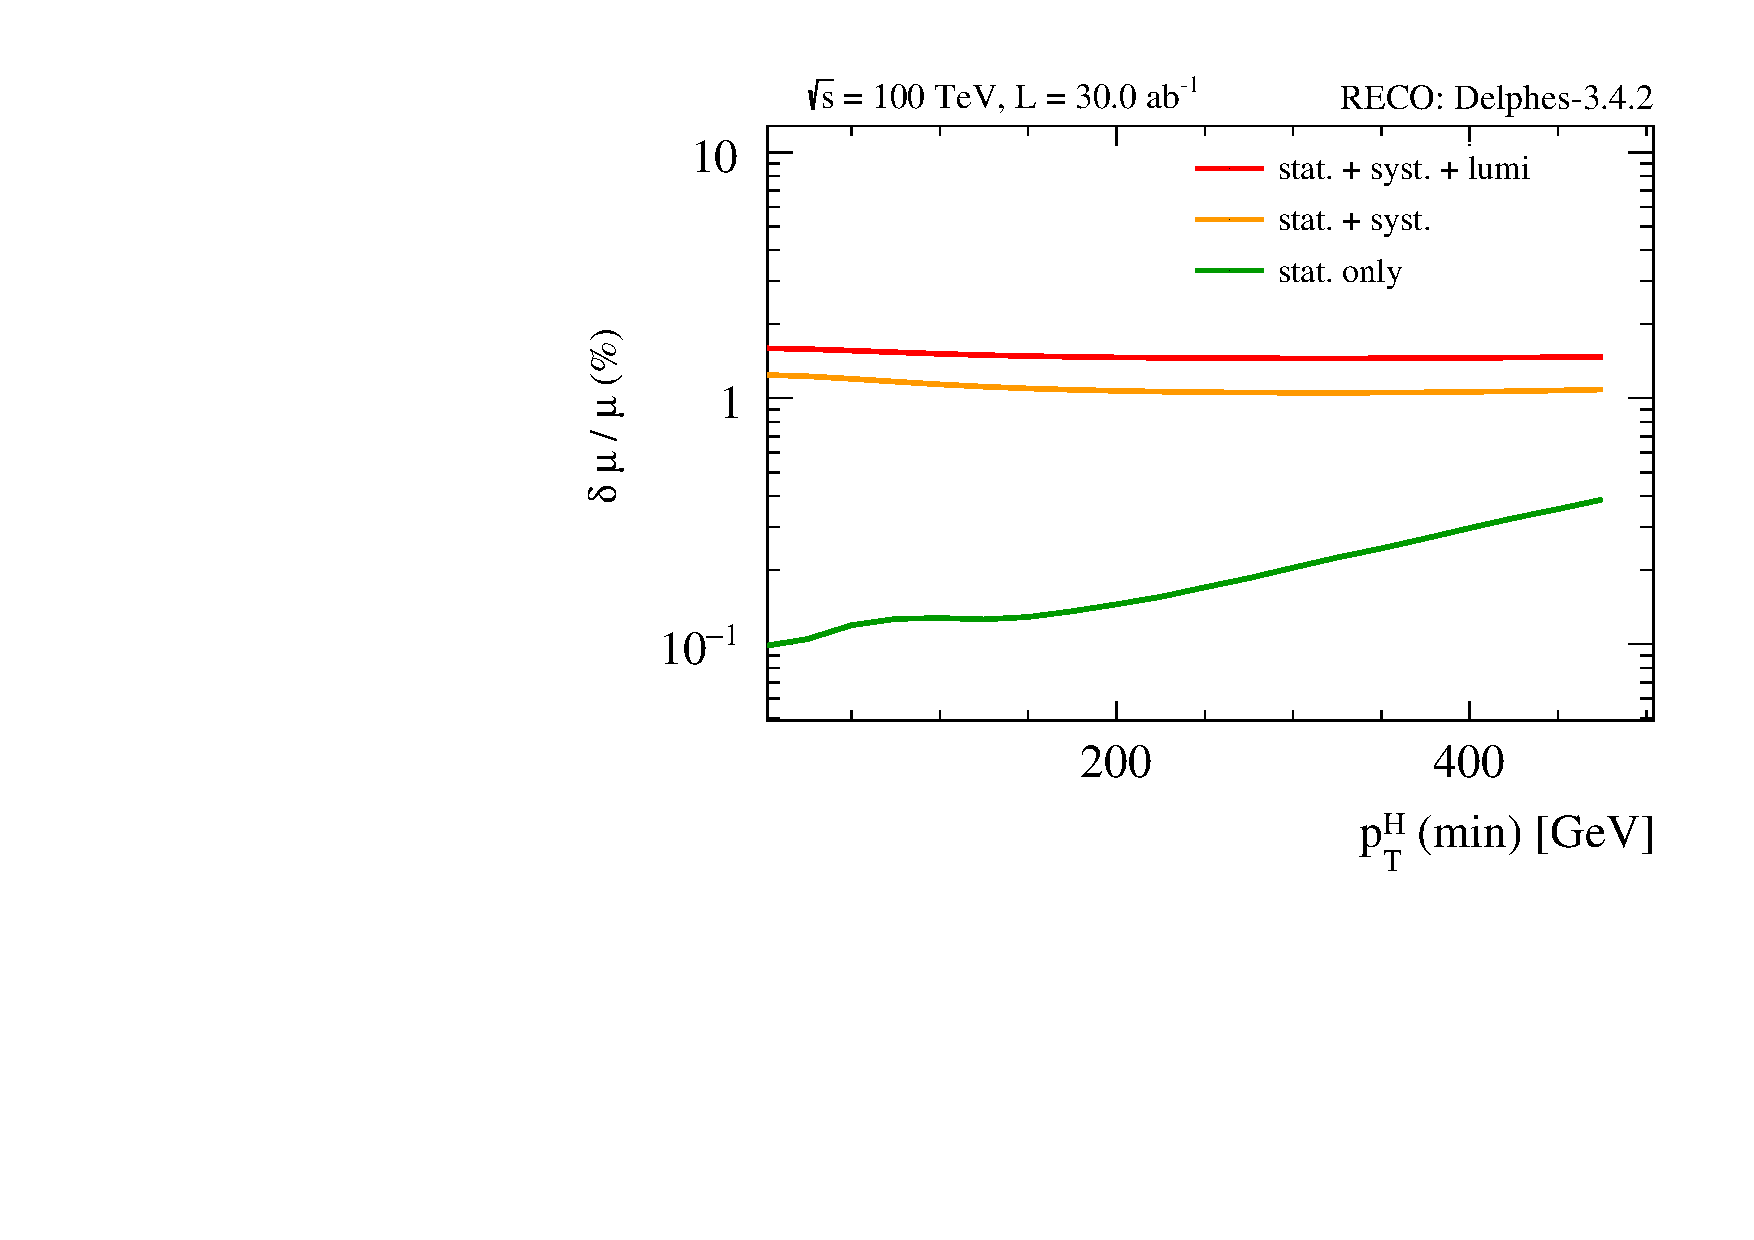
\includegraphics[width=0.45\textwidth]{\main/section1/img/hgg.pdf} .
%\end{verbatim}

%\begin{figure}[ht]
%\centering
%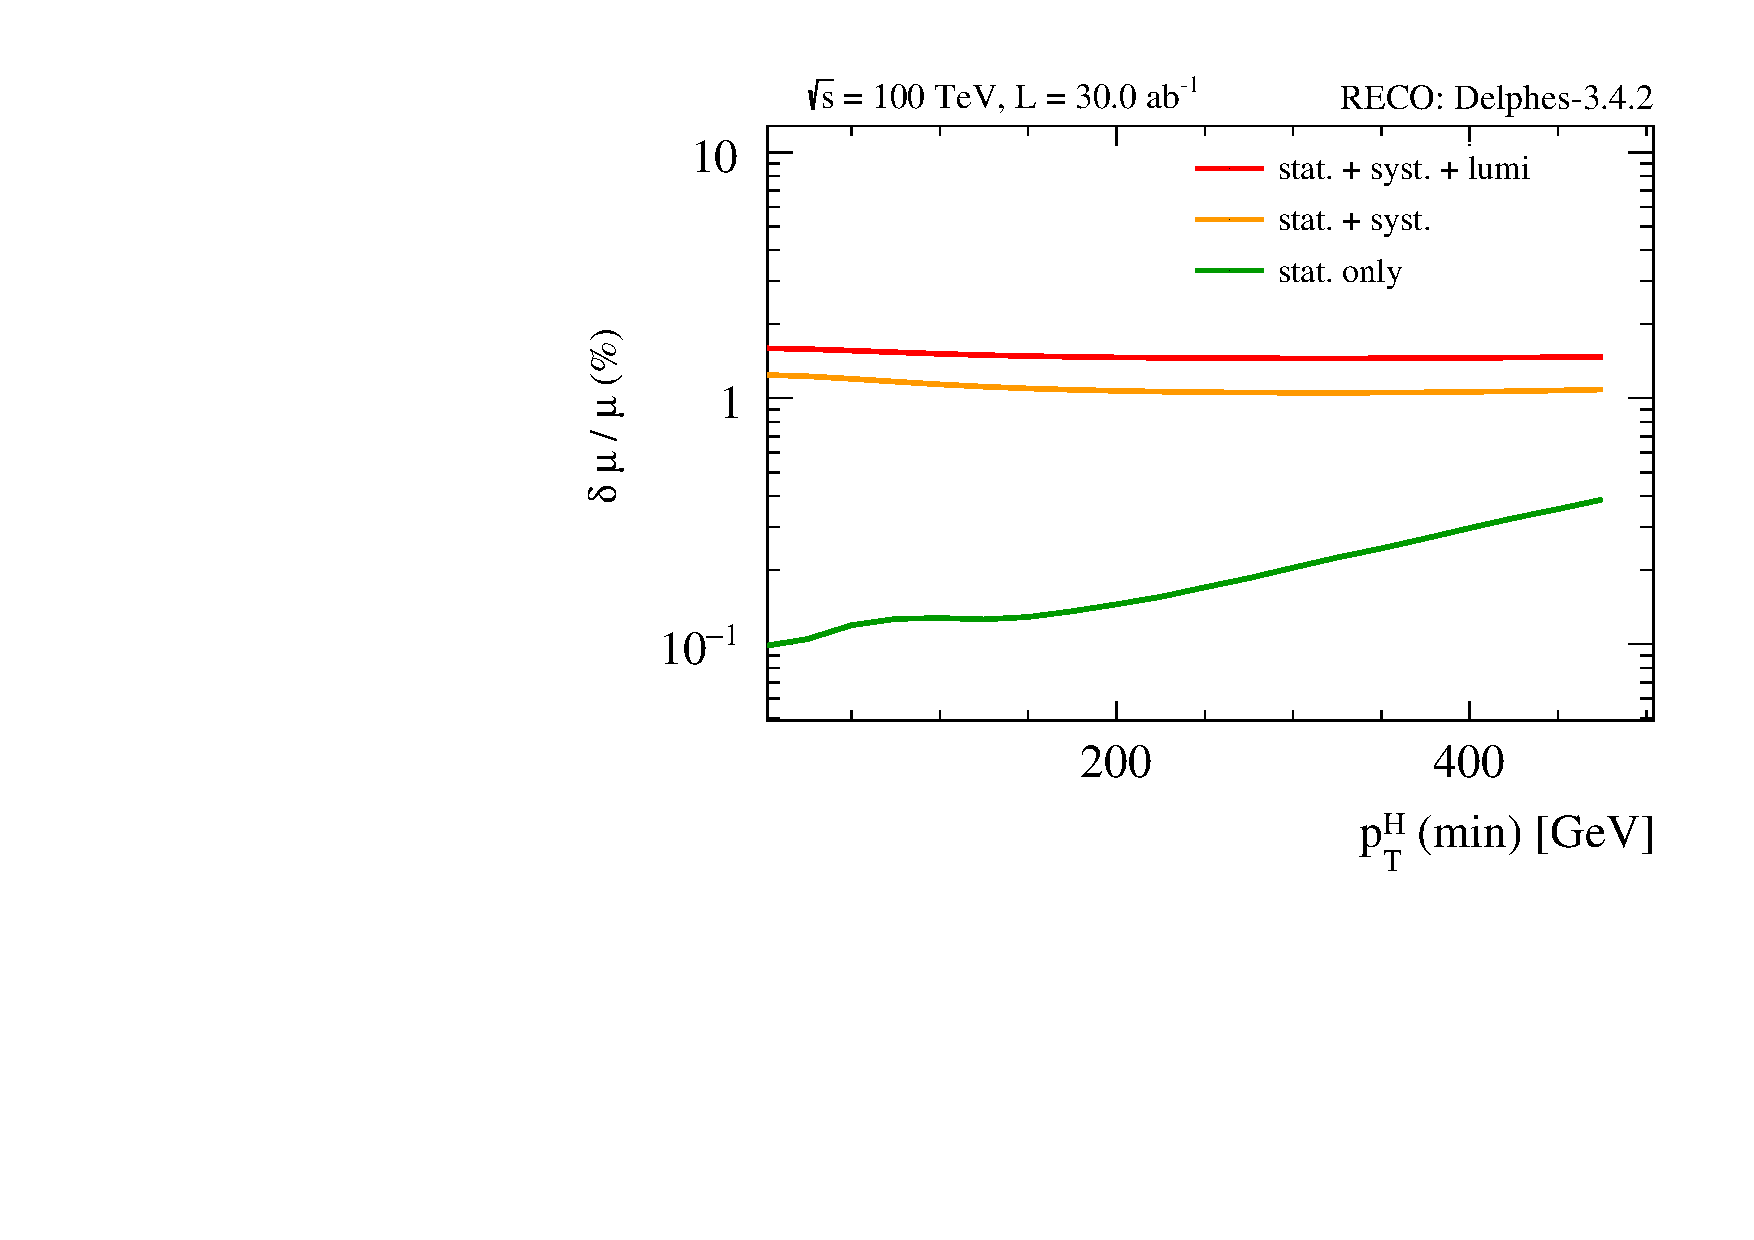
\includegraphics[width=0.75\textwidth]{\main/section1/img/hgg.pdf}
%\caption{Caption of the figure.}
%\label{fig:higgs}
%\end{figure}

%As for tables, please use the standard tabular environment, with the
%caption on top of the table. For cross referencing, try use lables
%such as
%\verb|\label{eq:eqname}|, \verb|\label{tab:tabname}| and
%\verb|\label{fig:figname}|. 

%If you need subsections, you can include them here directly, or input
%them as files, which can live in their own subdirectory. If including
%a subsection from a file, import them with the command
%\begin{verbatim}
%\subfile{\main/section1/sub1/mysubsec}
%\end{verbatim}
%where mysubsec.tex would start of course with the statement
%\verb|\begin{subsection}|.  In this case, make sure you define
%properly the path to figures and other files. This is crucial to
%guarantee compatibility of compilation of the whole Chapter and or the
%individual section. The fact that a Section compiles doesn't imply
%that the Chapter will compile, if paths are entered inaccurately. At
%this time I have not foreseen the ability to compile subsections
%standalone, I hope it is not necessary.

%\subfile{\main/section1/sub1/mysubsec}

\subfile{\main/section1/PerfAndSyst.tex}

\subsection{Implications for beyond the Standard Model theories}
\subfile{\main/section1/EFTintro.tex}
\subfile{\main/section1/IntroBSM.tex}



\end{document}
